\subsection{Lost lepton estimation}
\label{subsec:lostlept}
The lost lepton background is estimated from single lepton prompt (e,$\mu$) plus 
photon control regions. 
The definition of electrons and muons are the same as those used for the signal region 
veto defined in Section~\ref{sec:event-selection}.  Both the control regions require
exactly one lepton (e,$\mu$) and veto the opposite flavor lepton ($\mu$,e). In 
order to reduce the effect of signal contamination from signals with W bosons, for 
example, events in the control region are also required to satisfy $m_T=\sqrt{2p_{T}^{\ell}\ptmiss(1-cos(\dphi))}<100~\gev$. 
Figure \ref{fig:supp_Sim_MuGammaCS_mT_T5ttttZG} shows the distribution of $m_T$ for $\mu\gamma$ events
for SM processes and representative signal models (signal is scaled up by a factor of 10).
For standard model events, $m_T$ is constrained by the W boson mass, whereas for the signal,
missing transverse momentum from the gravitinos is included in $m_T$ .
The region with $m_T < 100$ \gev provides a background-enriched sample with very small signal contamination.
\begin{figure}[h!]
\centering
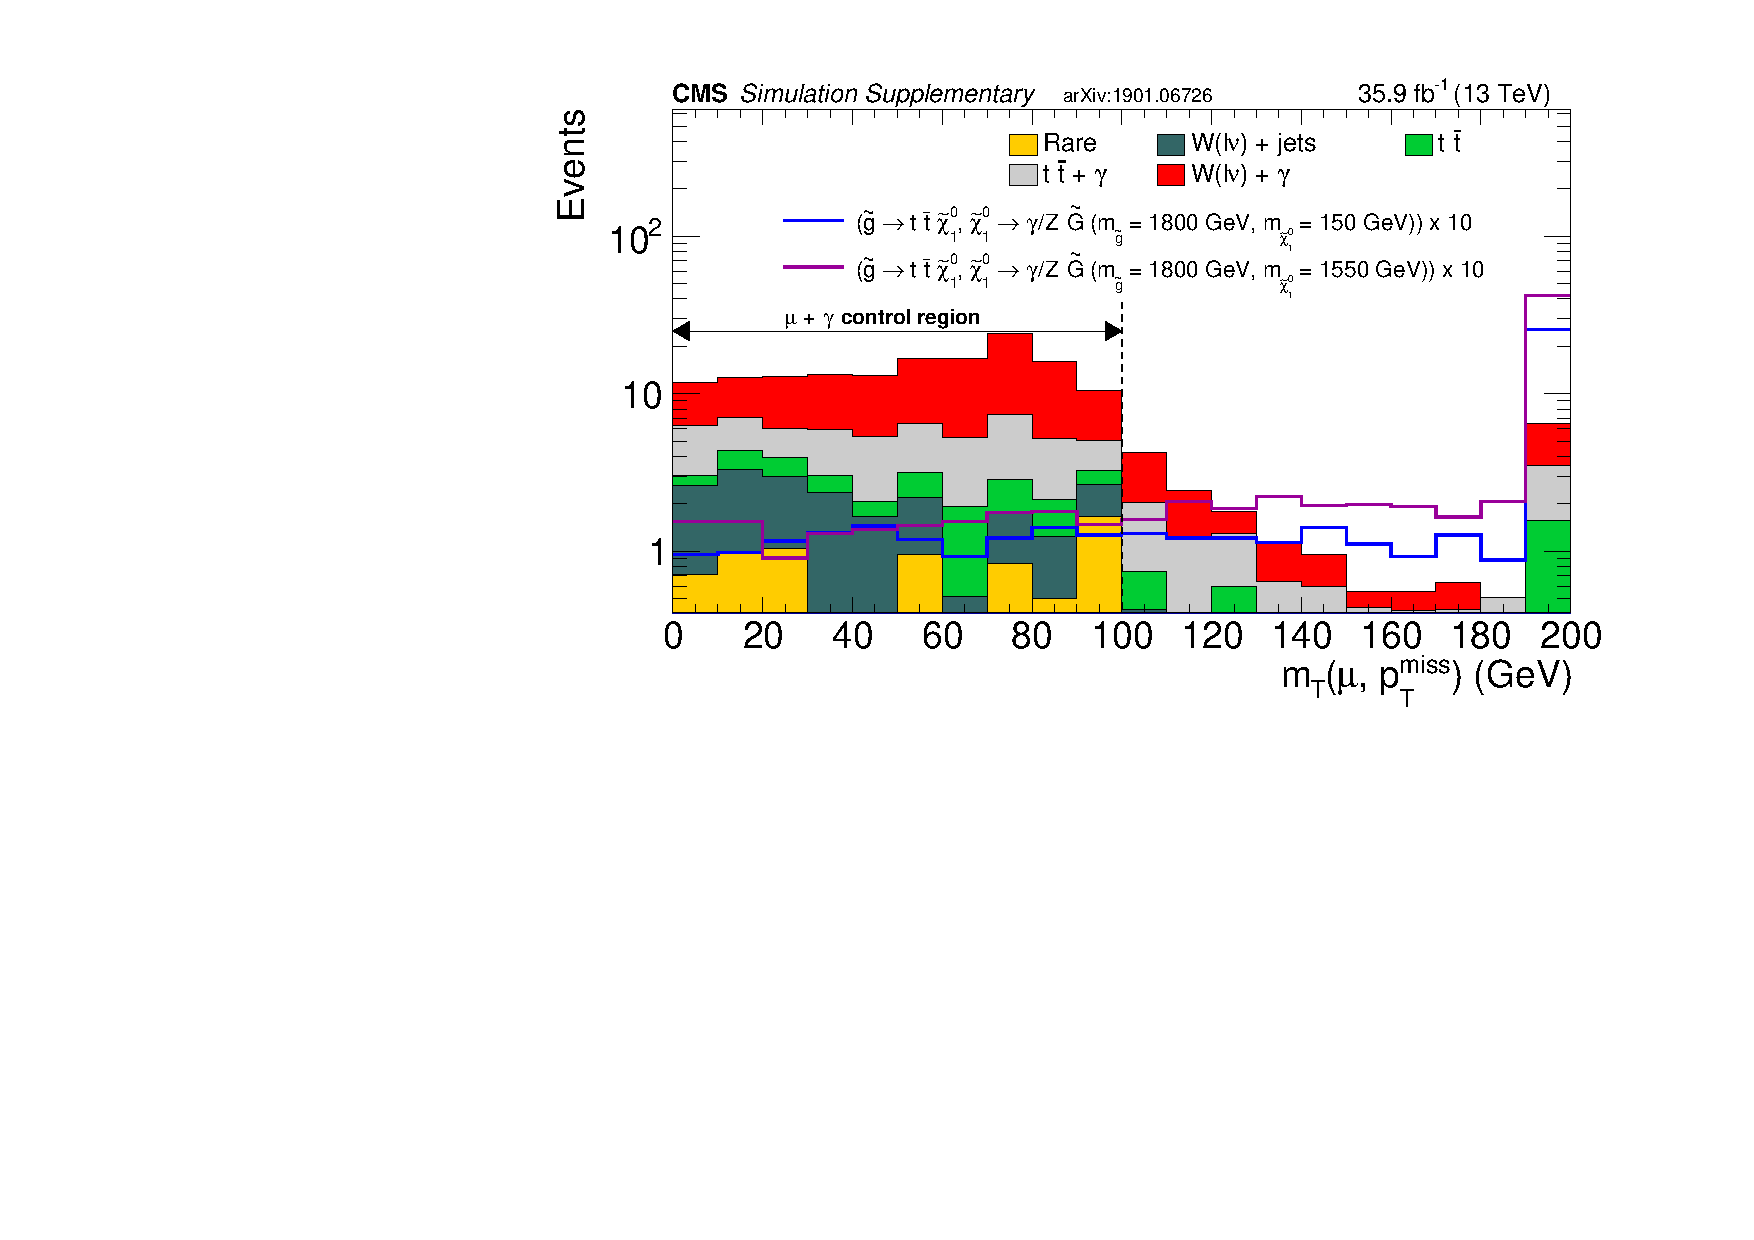
\includegraphics[width=0.8\linewidth]{../Figures/Chap3/anaPublic/supp_Sim_MuGammaCS_mT_T5ttttZG}
\captionsetup{width=.9\linewidth}
\caption[$m_T$ distribution for $\mu\gamma$ control region]{The transverse mass, $m_{T}$ distribution for $\mu\gamma$ events. Standard model processes are shown as filled histograms, representative signals of T5ttttZG model are shown as solid lines, and the signal is scaled up by a factor of 10 for better visualization.}
\label{fig:supp_Sim_MuGammaCS_mT_T5ttttZG}
\end{figure}

All other selections for the control region, isolated track vetos, \ST, \ptmiss, \nj,
and $\dphi$ are the same as the signal region. 
The control region events are triggered using the same triggers as the signal region
and the same trigger efficiency correction/efficiencies are applied.  

The method relies on weighting single lepton events. Event weights are derived
from simulations for electron and muon control samples separately.  The event 
weights are derived according to,
\begin{equation} \label{eq1}
\begin{split}
N_{lost-\ell}^{pred} & = N_{\ell}^{data}(\ptmiss,\nj,\nb) \cdot T^{\text{MC}}(\ptmiss,\nj,\nb)\\
\mathrm{where\ } T^{\text{MC}}(\ptmiss,\nj,\nb) & = N^{\text{MC}}_{lost-\ell}(\ptmiss,\nj,\nb) / N^{\text{MC}}_{\ell}(\ptmiss,\nj,\nb)
\end{split}
\end{equation}
$N_{\ell}^{data}$ and $T^{\text{MC}}$ are the observed yields in the control region
and the simulation-derived event weight for a corresponding search region.
For the muon ($\ell=\mu$) transfer factors, we include events with zero e,$\mu$, but at least one
hadronic-$\tau$ in the numerator of the transfer factor.

\begin{table}
\centering
\captionsetup{width=.9\linewidth}
\caption[TFs for lost lepton and \tauh]{Parameterization of transfer factors for lost-e and lost-$\mu+\tau_{\text{had}}$ events.}
\label{tab:lost_lepton_SF}
{\renewcommand{\arraystretch}{1.3}}% for the vertical padding
\begin{tabular}{c|c|c|c|c|c}
\hline
                          &            & \multicolumn{4}{c}{Event weight} \\ \cline{3-6}
                          &            & \multicolumn{2}{c|}{High-\dphi}   &\multicolumn{2}{c}{Low-\dphi} \\ \cline{3-6}
$N_{\mathrm{jets}}^{\mathrm{b-jets}}$       & \ptmiss    & Lost-e            & Lost-$\mu+\tau_{\text{had}}$ & Lost-e         & Lost-$\mu+\tau_{\text{had}}$ \\ \hline \hline
\multirow{2}{*}{$N_{2}^0$}& 100-150    & 0.55 $\pm$ 0.06 & 1.05 $\pm$ 0.07  & 0.23 $\pm$ 0.04 & 0.75 $\pm$ 0.10 \\ \cline{2-6}
                          & $\geq 150$ & 0.42 $\pm$ 0.04 & 0.84 $\pm$ 0.06  & 0.24 $\pm$ 0.04 & 0.66 $\pm$ 0.10 \\ \cline{1-6}
\multirow{2}{*}{$N_{3}^0$}& 100-150    & 0.30 $\pm$ 0.04 & 0.81 $\pm$ 0.06  & 0.20 $\pm$ 0.04 & 0.59 $\pm$ 0.12 \\ \cline{2-6}
                          & $\geq 150$ & 0.30 $\pm$ 0.04 & 0.67 $\pm$ 0.06  & 0.21 $\pm$ 0.04 & 0.54 $\pm$ 0.13 \\ \cline{1-6}
\multirow{2}{*}{$N_{4}^0$}& 100-150    & 0.29 $\pm$ 0.06 & 0.62 $\pm$ 0.10  & 0.26 $\pm$ 0.08 & 0.43 $\pm$ 0.12 \\ \cline{2-6}
						  & $\geq 150$ & 0.64 $\pm$ 0.06 & 1.23 $\pm$ 0.08  & 0.20 $\pm$ 0.04 & 0.67 $\pm$ 0.07 \\ \cline{1-6}
\multirow{2}{*}{$N_{5-6}^0$}& 100-150    & 0.30 $\pm$ 0.02 & 0.97 $\pm$ 0.05  & 0.16 $\pm$ 0.03 & 0.60 $\pm$ 0.07 \\ \cline{2-6}
                            & $\geq 150$ & 0.36 $\pm$ 0.03 & 0.79 $\pm$ 0.05  & 0.11 $\pm$ 0.02 & 0.43 $\pm$ 0.05 \\ \cline{1-6}
\multirow{2}{*}{$N_{\geq 7}^0$}& 100-150    & 0.25 $\pm$ 0.03 & 0.64 $\pm$ 0.04  & 0.17 $\pm$ 0.03 & 0.54 $\pm$ 0.07 \\ \cline{2-6}
                               & $\geq 150$ & 0.33 $\pm$ 0.08 & 0.73 $\pm$ 0.10  & 0.17 $\pm$ 0.05 & 0.59 $\pm$ 0.20 \\ \hline
\multirow{2}{*}{$N_{2-4}^{\geq 1}$}& 100-150 & 0.51 $\pm$ 0.05 & 0.87 $\pm$ 0.09  & 0.43 $\pm$ 0.06 & 0.98 $\pm$ 0.18 \\ \cline{2-6}
                          & $\geq 150$ & 0.39 $\pm$ 0.04 & 0.70 $\pm$ 0.07  & 0.21 $\pm$ 0.06 & 0.81 $\pm$ 0.15 \\ \cline{1-6}
\multirow{2}{*}{$N_{5-6}^{\geq 1}$}& 100-150    & 0.44 $\pm$ 0.08 & 0.64 $\pm$ 0.09  & 0.27 $\pm$ 0.09 & 0.45 $\pm$ 0.17 \\ \cline{2-6}
						  & $\geq 150$ & 0.57 $\pm$ 0.05 & 1.11 $\pm$ 0.10  & 0.27 $\pm$ 0.04 & 0.68 $\pm$ 0.10 \\ \cline{1-6}
\multirow{2}{*}{$N_{\geq 7}^{\geq 1}$} & 100-150    & 0.35 $\pm$ 0.04 & 0.79 $\pm$ 0.07  & 0.25 $\pm$ 0.04 & 0.54 $\pm$ 0.07 \\ \cline{2-6}
                          & $\geq 150$ & 0.36 $\pm$ 0.06 & 0.67 $\pm$ 0.10  & 0.25 $\pm$ 0.06 & 0.53 $\pm$ 0.10 \\\hline
\end{tabular}
\end{table}

Table~\ref{tab:lost_lepton_SF} shows the event weights for the two lost-lepton control regions.
These weights are typically 0.5 (0.75) for the e ($\mu$) control regions. 

To test the paremeterization of the event weights, the lost lepton method is evaluated 
on simulated data.  Figure~\ref{fig:lost_lepton_closure} shows comparisons of the predicted event yield
in each of the search regions and the true event yield from simulation for the electron
and $\mu+\tauh$ events.  The event weight parameterization is found to 
predict the true event yield for each of the search regions with the largest observed
deviation corresponding to a 30\% discrepancy, which is consistent with expectations
from statistical fluctuation only. 
The uncertainty on the event weights from limited MC statistics is propagated to the final predictions.
Any non-closure seen in the tighter \ptmiss region will be covered by the control sample statistical uncertainty in data.
%\textcolor{red}{Add 1D pull ../Figures/Chap3 for closure.}.

To model the uncertainty on the prediction due to limited statistics from the single 
lepton control regions, each prediction will have a prior distribution modeled by
a gamma distribution that uses the observed control region statistics and the average 
transfer factor.  The average transfer factor is defined to be the prediction 
divided by the raw observed control region event yield.  In bins where there are
no events observed, the average transfer factor is computed based on MC events 
yields.  

\begin{figure}
\centering
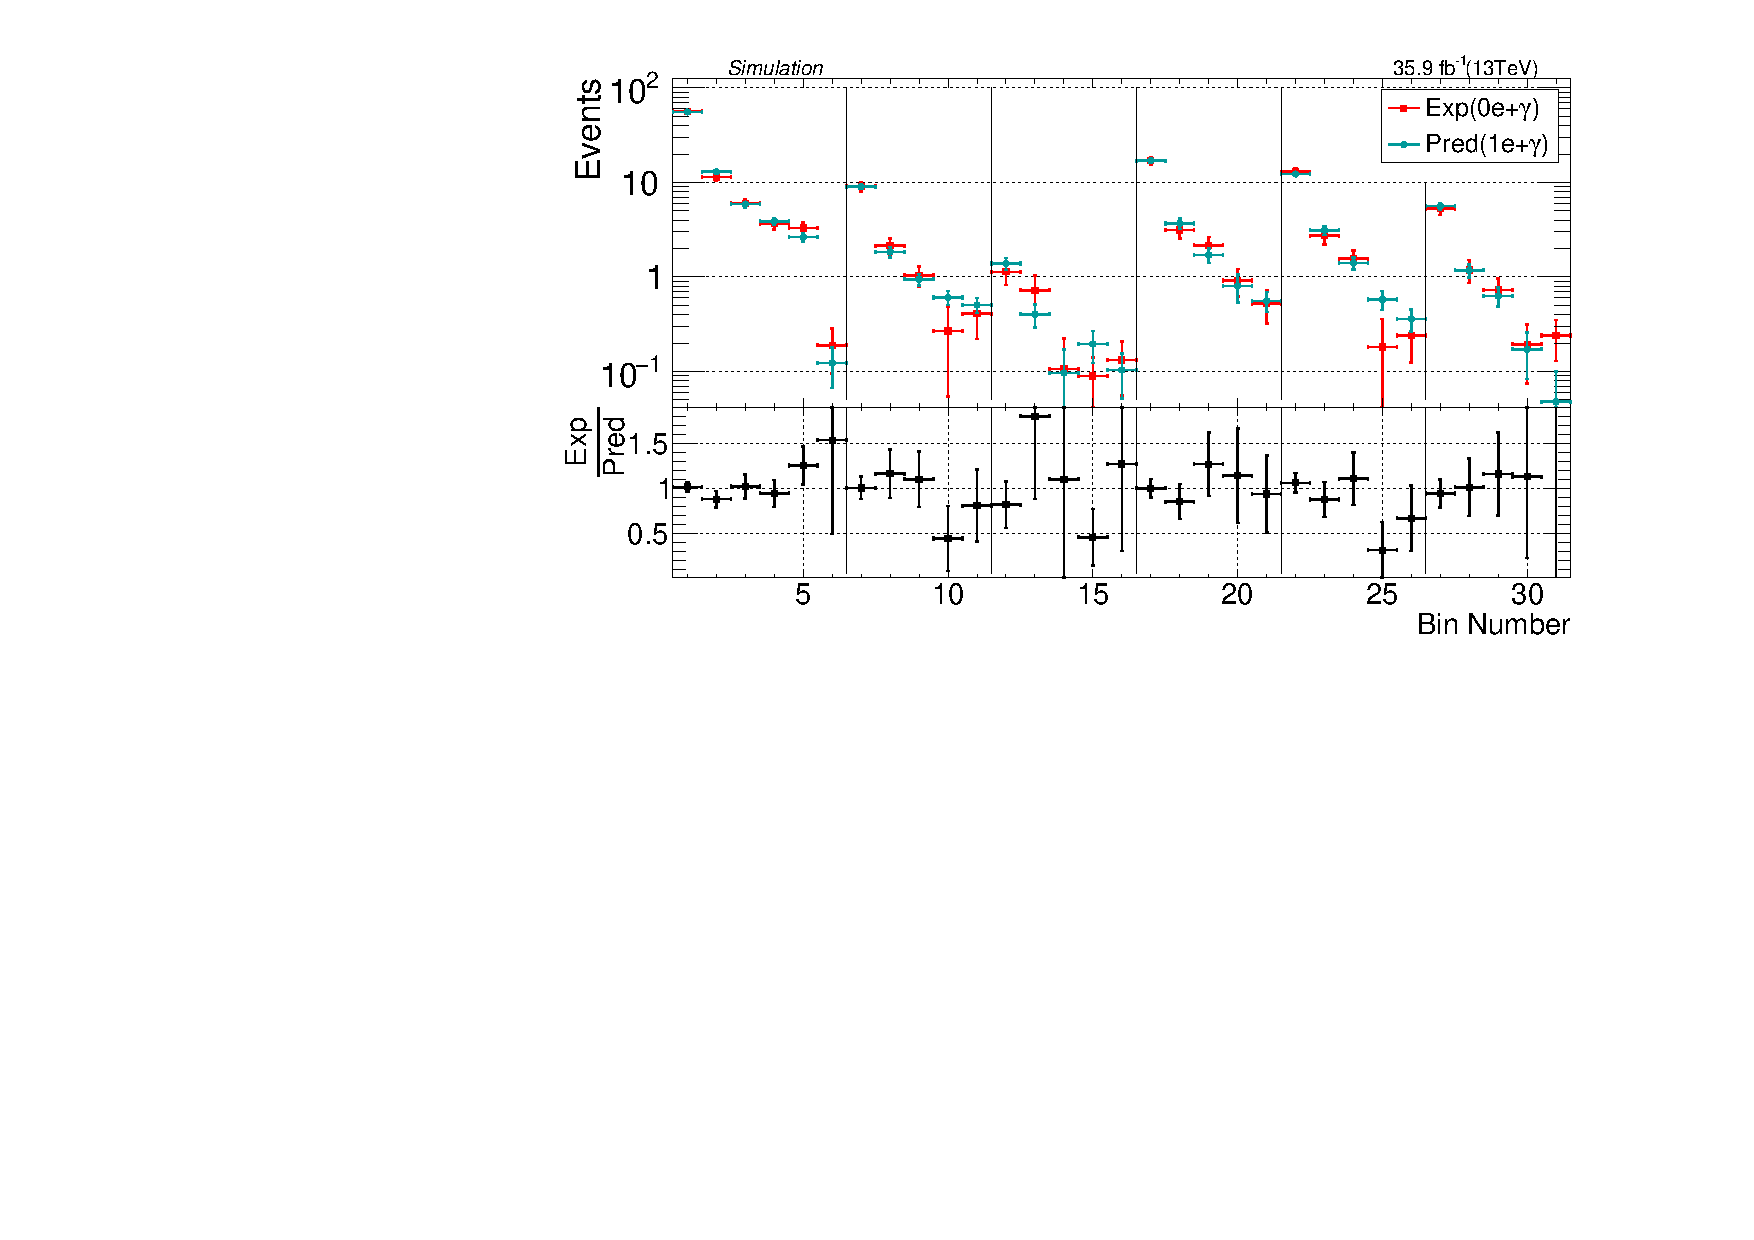
\includegraphics[width=0.48\linewidth]{../Figures/Chap3/SUSY_Photon_MET_JbJ_18Aug17/LostEle_Closure/AllSBins_v7_Ele0AllSBins_v7_Ele1.pdf}
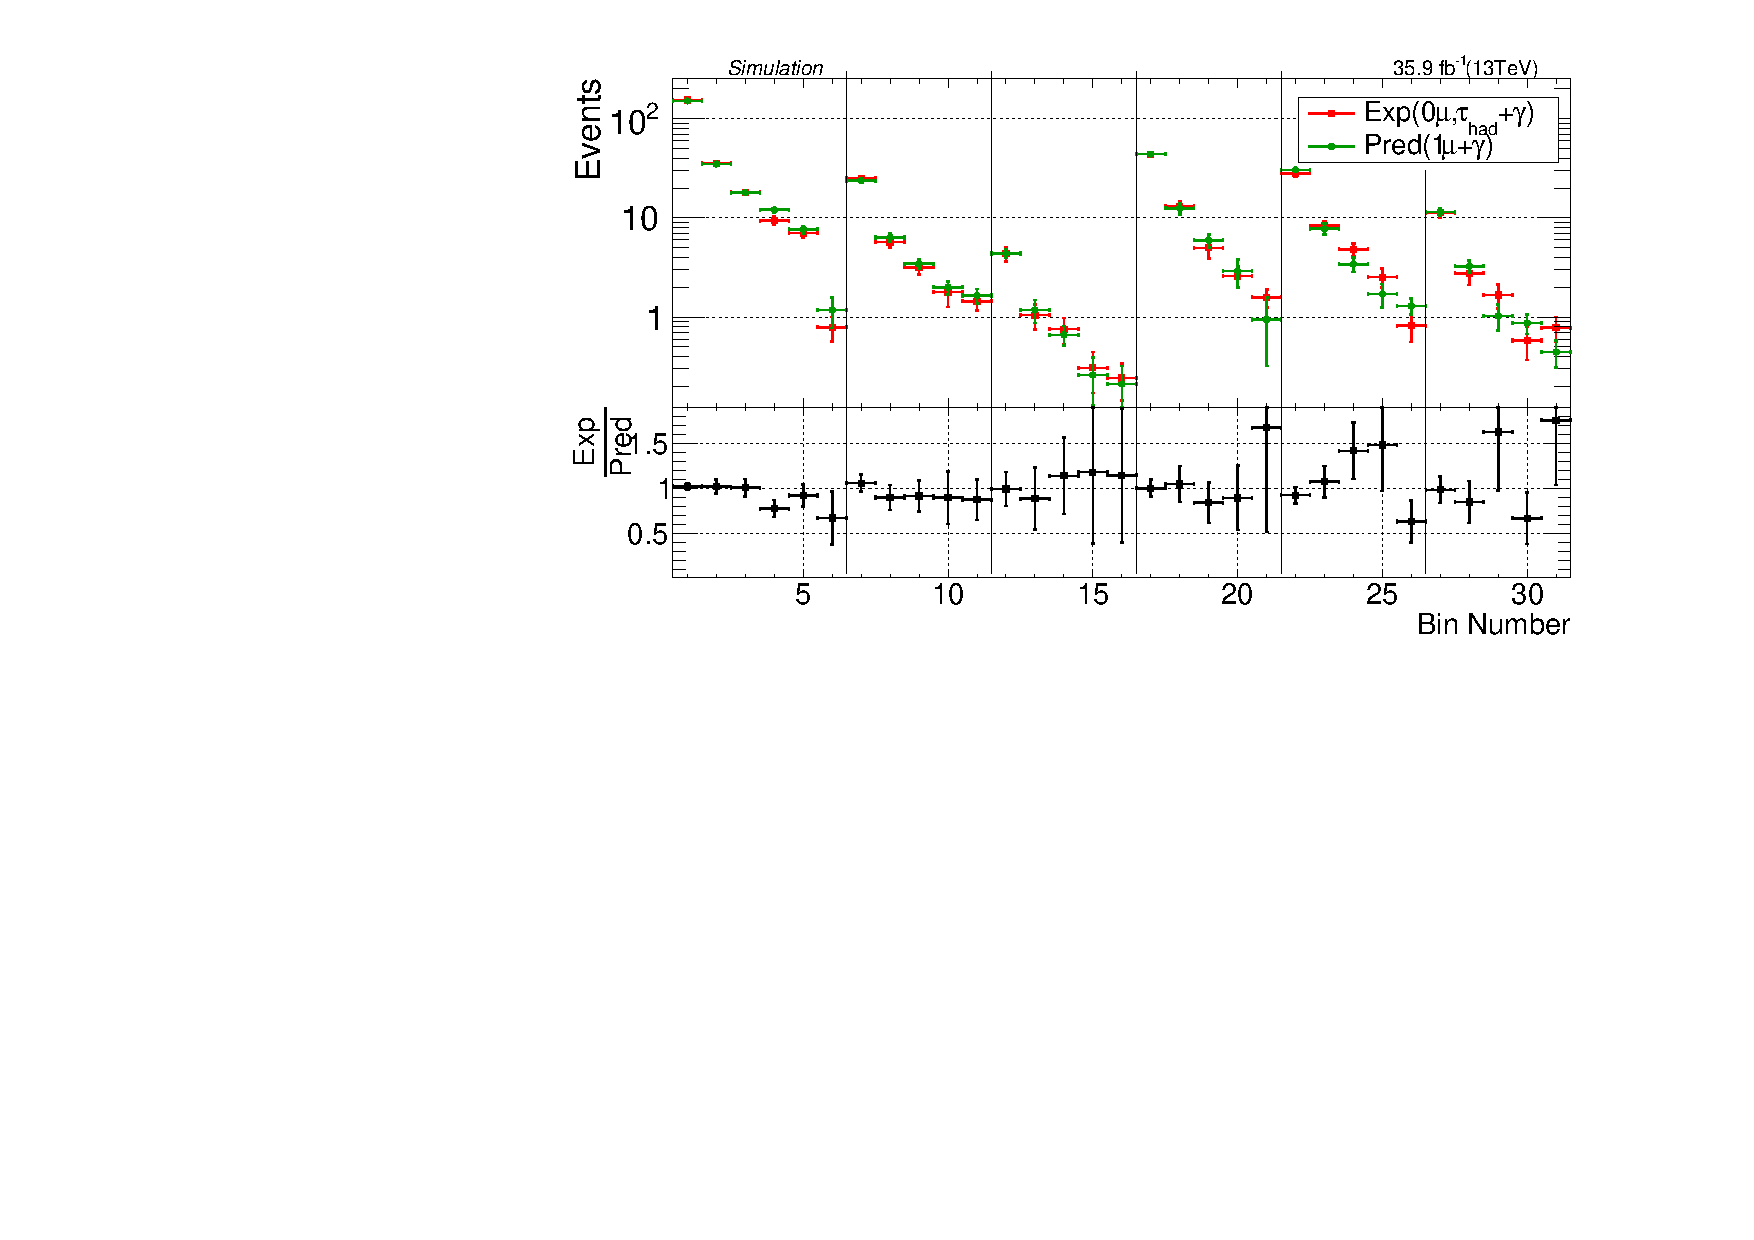
\includegraphics[width=0.48\linewidth]{../Figures/Chap3/SUSY_Photon_MET_JbJ_18Aug17/LostMu_Closure/AllSBins_v7_Mu0AllSBins_v7_Mu1.pdf}
\captionsetup{width=.9\linewidth}
\caption[Closure for lost lepton and \tauh]{Expected closure of lost electron (left) and lost $\mu+\tauh$ (right) predictions
where simulated event yields are treated like data.}
\label{fig:lost_lepton_closure}
\end{figure}

Other sources of systematic uncertainty correspond to effects related to:
\begin{itemize}
  \item lepton scale factors
  \item b-tagging scale factors
  \item PDF and scale uncertainties
  \item modeling of \mt in simulations
  \item modeling of colinear photons 
\end{itemize}

The PDF and scale uncertainties are studied by varying the MC weights according
to 101 and 9 weight sets respectively.  For each variation the average transfer factor for
all signal regions combined is computed.  
The maximum variation of the lost $\mu+\tauh$
average transfer factor is found to be 1.3\% and 0.7\% for the PDF and scale variations, 
respectively.  
The maximum variation of the lost $\mu$ average TF is found to be 1.3\% and 0.7\% for the PDF and scale variations respectively.
For the lost-e, 4.8\% and 1.0\% variations were found in TF because of the PDF and scale variations, respectively.
The maximum variation of these alternative weights is added as a systematic 
uncertainty on the lost-lepton and $\tauh$ prediction. A single nuisnace parameter
is used to model this uncertainty, correlating all signal regions and correlating
the effect of PDF and scale uncertainties for both lost-e and lost-$\mu+\tauh$
predictions. 

The effect of JEC uncertainties are studied by varying both jet \pt and \ptmiss.
This variation can cause events 
to migrate below the minimum \ptmiss or \ST thresholds, or above the maximum
\mt threshold for single lepton events.  No trends are observed versus 
the various signal region.  There is a 2\% (0.6\%) effect on the lost-e (lost-$\mu+\tauh$)
transfer factor, averaged over all signal regions.  The 2\% effect for the lost-e 
prediction is applied as a systematic uncertainty.  The effect on the lost-$\mu+\tauh$
prediction is neglected.
The same correlation model as used for the PDF and scale uncertainties is applied
for the JEC uncertainty systematic.  

The modeling of the \mt distribution is potentially effected by generator
level cuts in MC samples, but this effect is found to be
less than 1\% and is neglected.

The effect of uncertainties on the lepton scale factors are propagated
to the lost-e and lost-$\mu+\tauh$ transfer factors.  These are found to have
a 2\% effect, which is assumed to be correlated among common \ptmiss bins.  

Finally the effect of b-tagging scale factor uncertainties was checked.  
It was found to have $<1\%$ effect on the lost-lepton transfer factors
and is neglected. 

Comparisons between simulation and data for single lepton events show
a systematic mismodeling of events with small angle between the e/$\mu$
and the photon.  This is due to generator level cuts on the angle between
photons and partons, in Madgraph W/$t\bar{t}+\gamma$ samples, of $\Delta R<0.5$,
which is not well modeled by pythia W/$t\bar{t}$+jets samples. Figure~\ref{fig:lost_ell_dR_dist}
shows the $\Delta R(e,\gamma)$ and $\Delta R(\mu,\gamma)$ distributions.  
The region $\Delta R(e,\gamma)<0.2$ is excluded due to the photon/electron
isolation cuts. To assess the effect of the missing low $\Delta R$
phase space, the average transfer factor is derived for events with 
$\Delta R>0.5$ and compared to the average transfer factor computed 
with all events.  The effect is found to be a 12\%
effect on the lost-e transfer factor and $<1\%$ on the 
lost-$\mu+\tauh$ transfer factor.  Since no trends are found versus various 
signal regions, a flat 12\% uncertainty is applied
to lost-e prediction.  No systematic uncertainty is applied to
the lost-$\mu+\tauh$ prediction.

\begin{figure}
\centering
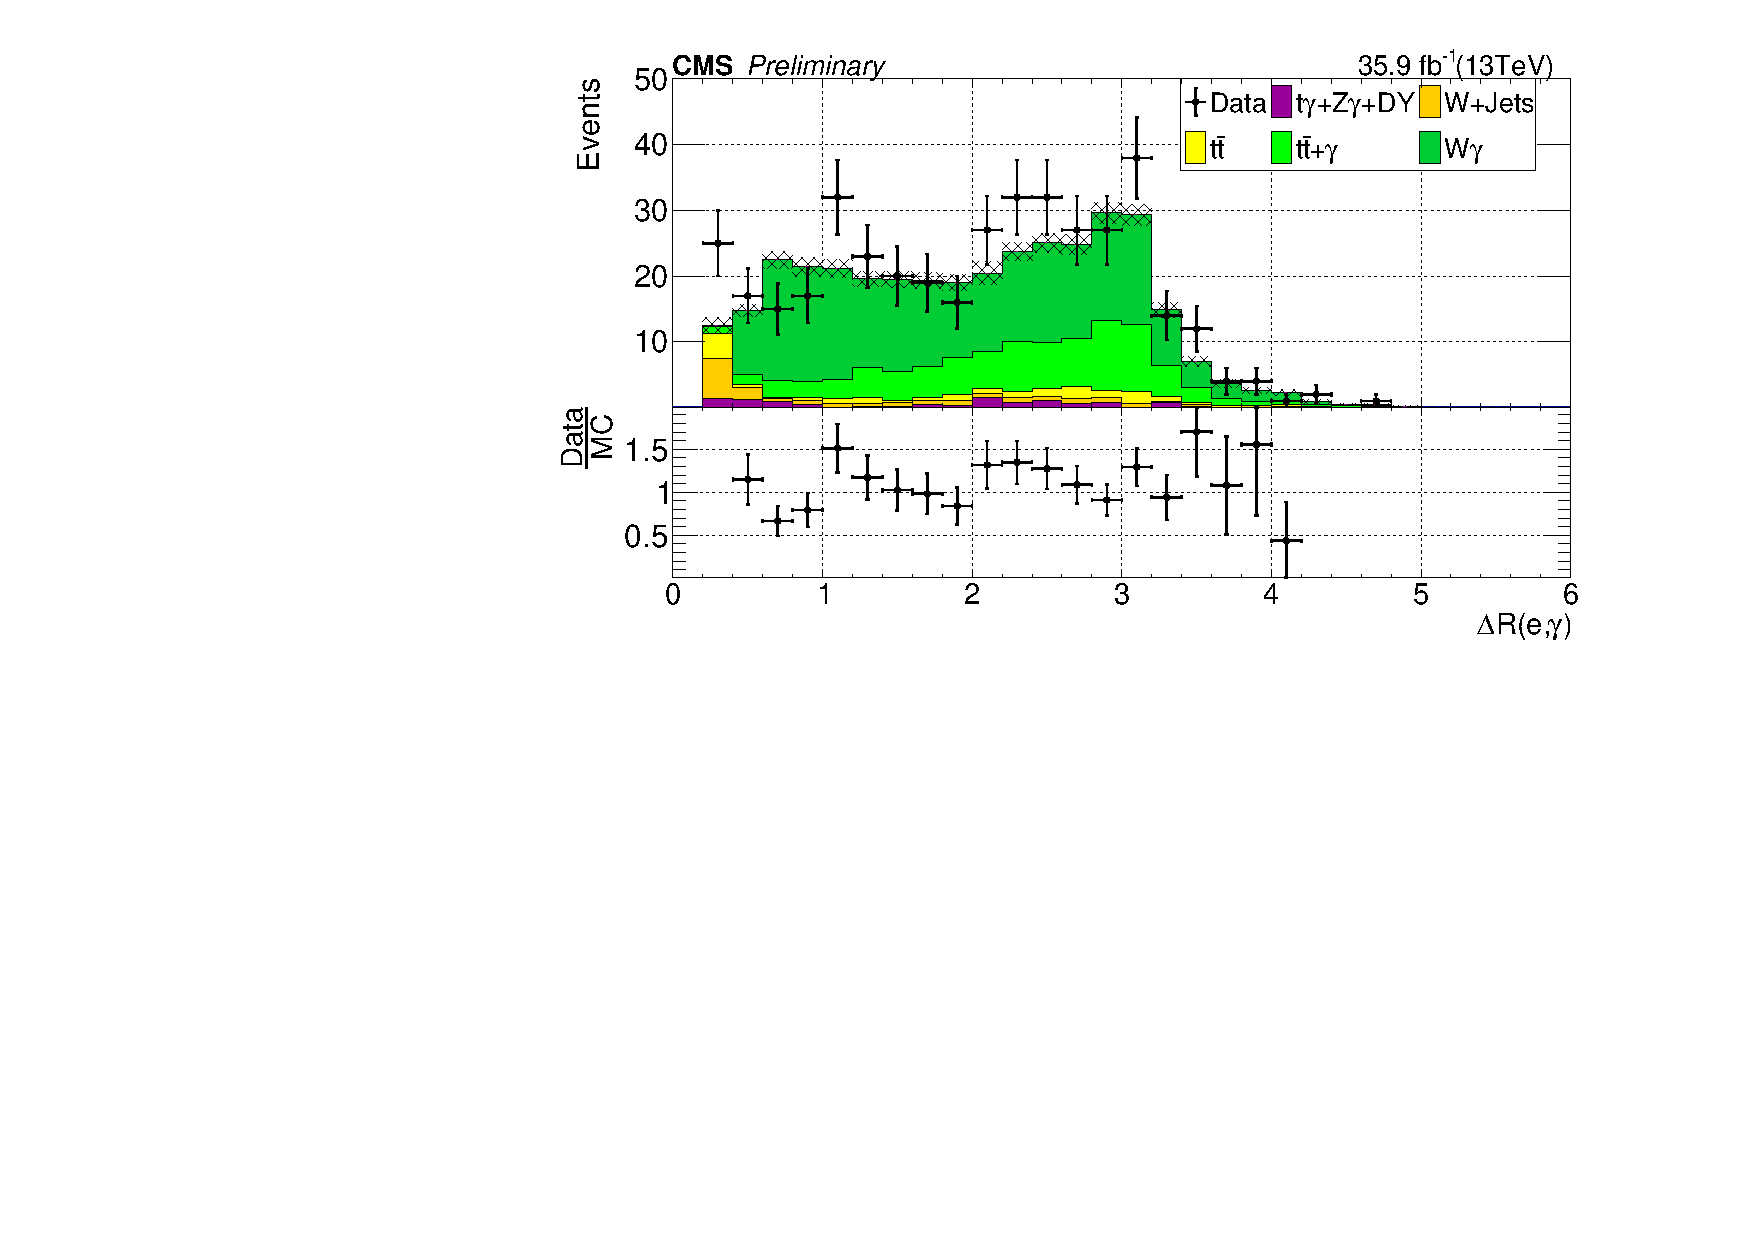
\includegraphics[width=0.48\linewidth]{../Figures/Chap3/lost_lepton/lostElectronDeltaR.pdf}
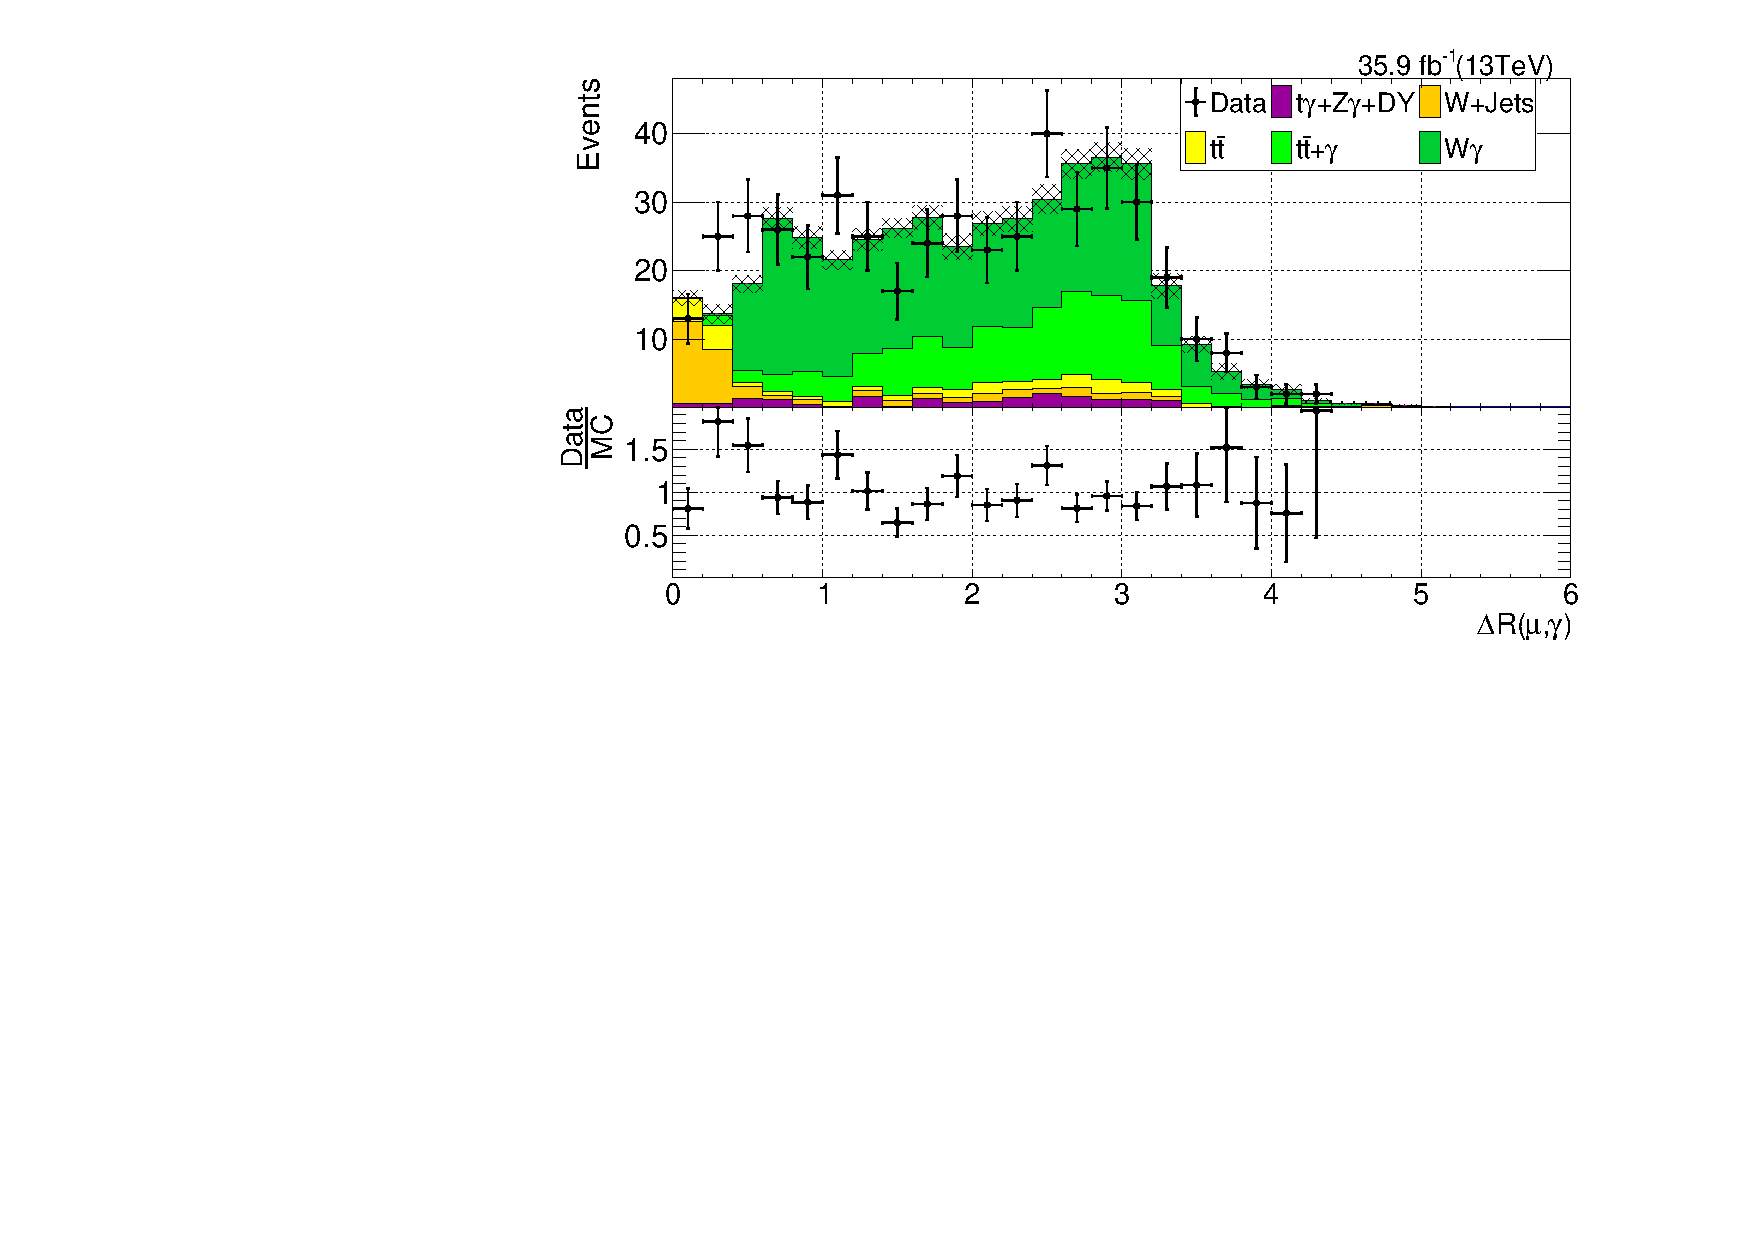
\includegraphics[width=0.48\linewidth]{../Figures/Chap3/lost_lepton/lostMuonDeltaR.pdf}
\captionsetup{width=.9\linewidth}
\caption[$\Delta R(\ell,\gamma)$ for $\mu\gamma$ and $e\gamma$ CRs]{Distribution of $\Delta R(\ell,\gamma)$ for single
electron (left) and single muon (right) events.}
\label{fig:lost_ell_dR_dist}
\end{figure}

The observed event yields and the corresponding predictions are shown in Table~\ref{tab:lostLeptonPredictions} (for high \dphi) and Table~\ref{tab:lostLeptonPredictions_LDP} (for low \dphi) of appendix \ref{AppendixB}. 
Comparisons of the observed yields and expected MC yields for the $e+\gamma$ and $\mu+\gamma$ control 
regions in Figures~\ref{fig:lost_mu_CR_dist} and~\ref{fig:lost_e_CR_dist} of appendix \ref{AppendixC}.

